\documentclass[aspectratio=169,11pt]{beamer}

% ============================================
% PACKAGES ET CONFIGURATION
% ============================================
\usepackage[utf8]{inputenc}
\usepackage[T1]{fontenc}
\usepackage[french]{babel}
\usepackage{amsmath}
\usepackage{amssymb}
\usepackage{amsthm}
\usepackage{graphicx}
\usepackage{algorithm}
\usepackage{algorithmic}
\usepackage{booktabs}
\usepackage{multirow}
\usepackage{array}
\usepackage{xcolor}
\usepackage{hyperref}

% ============================================
% THÈME ET COULEURS
% ============================================
% Thème moderne et épuré : Darmstadt (alternative : Berlin, Warsaw)
\usetheme{Darmstadt}
\usecolortheme{default}

% Couleurs personnalisées
\definecolor{bleu}{RGB}{0,102,204}
\definecolor{rouge}{RGB}{204,0,51}
\definecolor{vert}{RGB}{0,153,51}

% Réduction des espacements pour plus de contenu
\setbeamertemplate{itemize item}[circle]
\setbeamertemplate{itemize subitem}[triangle]
\setlength{\leftmargini}{0.5cm}
\setbeamersize{text margin left=0.5cm,text margin right=0.5cm}

% ============================================
% INFORMATIONS DE LA PRÉSENTATION
% ============================================
\title[Intégration Numérique]{Comparaison de Méthodes d'Intégration Numérique}
\subtitle{Analyse Comparative de 5 Méthodes sur 4 Exemples}
\author{CISSE BRAHIMA}
\institute{L'UNIVERSITÉ NANGUI ABROGOUA (UNA)}
\date{\today}

% ============================================
% COMMANDES PERSONNALISÉES
% ============================================
\newcommand{\R}{\mathbb{R}}
\newcommand{\N}{\mathbb{N}}

% ============================================
% DÉBUT DU DOCUMENT
% ============================================
\begin{document}

% ============================================
% PAGE DE TITRE
% ============================================
\begin{frame}
\titlepage
\end{frame}

% ============================================
% TABLE DES MATIÈRES
% ============================================
\begin{frame}{Plan de la Présentation}
\tableofcontents
\end{frame}

% ============================================
% SECTION 1: INTRODUCTION
% ============================================
\section{Introduction}

\begin{frame}{Contexte et Motivation}
\vspace{-0.2cm}
\begin{block}{Problématique}
\small
\begin{itemize}
\item Calcul d'intégrales définies sans solution analytique
\item Besoin de méthodes numériques efficaces et précises
\item Compromis entre précision et temps de calcul
\end{itemize}
\end{block}

\vspace{-0.1cm}
\begin{block}{Objectifs}
\small
\begin{itemize}
\item Comparer 5 méthodes d'intégration numérique
\item Tester sur 4 types de fonctions différents
\item Analyser les performances (erreur et temps)
\item Identifier les domaines d'application optimaux
\end{itemize}
\end{block}
\end{frame}

\begin{frame}{Structure du Projet}
\begin{columns}
\begin{column}{0.5\textwidth}
\textbf{Architecture du code :}
\begin{itemize}
\item \texttt{methods.py} : Implémentation des 5 méthodes
\item \texttt{examples.py} : 4 fonctions de test
\item \texttt{compute.py} : Exécution et collecte des résultats
\item \texttt{plots.py} : Génération des graphiques
\item \texttt{main.py} : Point d'entrée principal
\end{itemize}
\end{column}

\begin{column}{0.5\textwidth}
\textbf{Méthodes implémentées :}
\begin{enumerate}
\item Gauss-Legendre
\item Gauss-Laguerre
\item Gauss-Chebyshev
\item Simpson
\item Spline cubique
\end{enumerate}
\end{column}
\end{columns}
\end{frame}

% ============================================
% SECTION 2: MÉTHODES D'INTÉGRATION
% ============================================
\section{Méthodes d'Intégration Numérique}

\begin{frame}{Méthode de Gauss-Legendre}
\vspace{-0.2cm}
\begin{block}{Principe}
\small Quadrature basée sur les polynômes orthogonaux de Legendre
\end{block}

\vspace{-0.15cm}
\begin{block}{Formule mathématique}
\small
Pour une intégrale sur $[a,b]$ :
\begin{equation}
\int_a^b f(x) \, dx \approx \frac{b-a}{2} \sum_{i=1}^n w_i f(t_i)
\end{equation}
où :
\begin{itemize}
\item $t_i = \frac{b-a}{2}x_i + \frac{a+b}{2}$ (transformation $[-1,1] \to [a,b]$)
\item $(x_i, w_i)$ : racines et poids de Legendre dans $[-1,1]$
\end{itemize}
\end{block}

\vspace{-0.15cm}
\begin{block}{Caractéristiques}
\small
\begin{itemize}
\item Domaine : Intervalles finis $[a,b]$
\item Précision : Très élevée (ordre $2n$)
\item Complexité : $O(n)$
\end{itemize}
\end{block}
\end{frame}

\begin{frame}{Algorithme : Gauss-Legendre}
\vspace{-0.3cm}
\begin{algorithm}[H]
\caption{Quadrature de Gauss-Legendre}
\small
\begin{algorithmic}[1]
\REQUIRE Fonction $f$, bornes $a$, $b$, ordre $n$
\ENSURE Approximation de $\int_a^b f(x) dx$
\STATE Calculer $(x_i, w_i) = \text{leggauss}(n)$ dans $[-1,1]$
\STATE Transformer : $t_i = \frac{b-a}{2}x_i + \frac{a+b}{2}$ pour $i=1,\ldots,n$
\STATE Évaluer $f(t_i)$ pour $i=1,\ldots,n$
\STATE Calculer $I = \frac{b-a}{2} \sum_{i=1}^n w_i f(t_i)$
\RETURN $I$
\end{algorithmic}
\end{algorithm}
\end{frame}

\begin{frame}{Méthode de Gauss-Laguerre}
\vspace{-0.2cm}
\begin{block}{Principe}
\small Adaptée aux intégrales sur $[0, +\infty)$ avec poids exponentiel
\end{block}

\vspace{-0.15cm}
\begin{block}{Formule mathématique}
\small
Pour des intégrales de la forme :
\begin{equation}
\int_0^{+\infty} f(x) e^{-x} \, dx \approx \sum_{i=1}^n w_i f(x_i)
\end{equation}
où $(x_i, w_i)$ sont les racines et poids de Laguerre.
\end{block}

\vspace{-0.15cm}
\begin{block}{Application}
\small
Pour calculer $\int_0^{+\infty} g(x) dx$ :
\begin{equation}
\int_0^{+\infty} g(x) dx = \int_0^{+\infty} [g(x) e^x] e^{-x} dx
\end{equation}
On applique la quadrature à $f(x) = g(x) e^x$.
\end{block}
\end{frame}

\begin{frame}{Méthode de Gauss-Chebyshev}
\vspace{-0.2cm}
\begin{block}{Principe}
\small Quadrature avec poids $1/\sqrt{1-x^2}$ sur $[-1,1]$
\end{block}

\vspace{-0.15cm}
\begin{block}{Formule mathématique}
\small
Pour des intégrales de la forme :
\begin{equation}
\int_{-1}^{1} \frac{f(x)}{\sqrt{1-x^2}} \, dx \approx \frac{\pi}{n} \sum_{k=1}^n f(x_k)
\end{equation}
où les points de Chebyshev sont :
\begin{equation}
x_k = \cos\left(\frac{(2k-1)\pi}{2n}\right), \quad k=1,\ldots,n
\end{equation}
\end{block}

\vspace{-0.15cm}
\begin{block}{Transformation de domaine}
\small
Pour un domaine $[a,b] \neq [-1,1]$, transformation affine :
\begin{equation}
t = \frac{b-a}{2}(x+1) + a
\end{equation}
\end{block}
\end{frame}

\begin{frame}{Méthode de Simpson}
\vspace{-0.2cm}
\begin{block}{Principe}
\small Approximation par paraboles (méthode composite)
\end{block}

\vspace{-0.15cm}
\begin{block}{Formule mathématique}
\small
Pour $n$ sous-intervalles pairs sur $[a,b]$ avec $h = \frac{b-a}{n}$ :
\begin{equation}
\int_a^b f(x) dx \approx \frac{h}{3} \left[ f(x_0) + f(x_n) + 4\sum_{i \text{ impair}} f(x_i) + 2\sum_{i \text{ pair}} f(x_i) \right]
\end{equation}
où $x_i = a + ih$ pour $i=0,\ldots,n$.
\end{block}

\vspace{-0.15cm}
\begin{block}{Caractéristiques}
\small
\begin{itemize}
\item Domaine : Intervalles finis quelconques
\item Précision : Ordre 4 (erreur $\sim h^4$)
\item Robustesse : Très bonne pour fonctions régulières
\item Complexité : $O(n)$
\end{itemize}
\end{block}
\end{frame}

\begin{frame}{Algorithme : Simpson Composite}
\vspace{-0.3cm}
\begin{algorithm}[H]
\caption{Méthode de Simpson Composite}
\small
\begin{algorithmic}[1]
\REQUIRE Fonction $f$, bornes $a$, $b$, nombre de sous-intervalles $n$
\ENSURE Approximation de $\int_a^b f(x) dx$
\IF{$n$ est impair}
    \STATE $n \leftarrow n+1$ \COMMENT{Simpson nécessite $n$ pair}
\ENDIF
\STATE $h \leftarrow (b-a)/n$
\STATE $x \leftarrow [a, a+h, a+2h, \ldots, b]$ \COMMENT{$n+1$ points}
\STATE $y \leftarrow f(x)$ \COMMENT{Évaluation de la fonction}
\STATE $I \leftarrow \frac{h}{3} \left[ y[0] + y[n] + 4\sum_{i \text{ impair}} y[i] + 2\sum_{i \text{ pair interne}} y[i] \right]$
\RETURN $I$
\end{algorithmic}
\end{algorithm}
\end{frame}

\begin{frame}{Méthode Spline Cubique}
\vspace{-0.2cm}
\begin{block}{Principe}
\small Interpolation par splines cubiques puis intégration exacte
\end{block}

\vspace{-0.15cm}
\begin{block}{Approche}
\small
\begin{enumerate}
\item Évaluer $f$ en $n$ points équidistants : $x_i = a + i\frac{b-a}{n-1}$
\item Construire une spline cubique $S(x)$ interpolant $(x_i, f(x_i))$
\item Intégrer exactement la spline :
\begin{equation}
\int_a^b f(x) dx \approx \int_a^b S(x) dx
\end{equation}
\end{enumerate}
\end{block}

\vspace{-0.15cm}
\begin{block}{Caractéristiques}
\small
\begin{itemize}
\item Précision : Très élevée pour fonctions lisses (ordre 4)
\item Complexité : $O(n^2)$ construction, $O(n)$ intégration
\item Inconvénient : Plus coûteuse en temps de calcul
\end{itemize}
\end{block}
\end{frame}

\begin{frame}{Algorithme : Intégration par Spline}
\vspace{-0.3cm}
\begin{algorithm}[H]
\caption{Intégration par Spline Cubique}
\small
\begin{algorithmic}[1]
\REQUIRE Fonction $f$, bornes $a$, $b$, nombre de points $n$
\ENSURE Approximation de $\int_a^b f(x) dx$
\STATE $x \leftarrow \text{linspace}(a, b, n)$ \COMMENT{Points équidistants}
\STATE $y \leftarrow f(x)$ \COMMENT{Évaluation}
\IF{$\exists i : y[i]$ n'est pas fini}
    \RETURN NaN \COMMENT{Gestion des singularités}
\ENDIF
\STATE $S \leftarrow \text{CubicSpline}(x, y)$ \COMMENT{Construction de la spline}
\STATE $I \leftarrow S.\text{integrate}(a, b)$ \COMMENT{Intégration exacte}
\RETURN $I$
\end{algorithmic}
\end{algorithm}
\end{frame}

% ============================================
% SECTION 3: EXEMPLES DE FONCTIONS
% ============================================
\section{Exemples de Fonctions Testées}

\begin{frame}{Fonction Chebyshev}
\vspace{-0.2cm}
\begin{block}{Définition}
\small
\begin{equation}
f(x) = \frac{1}{\sqrt{1-x^2}}, \quad x \in [-0.9, 0.9]
\end{equation}
\end{block}

\vspace{-0.15cm}
\begin{block}{Caractéristiques}
\small
\begin{itemize}
\item Singularités aux bornes $\pm 1$ (hors du domaine)
\item Poids naturel : $1/\sqrt{1-x^2}$
\item Méthode attendue : Gauss-Chebyshev devrait exceller
\end{itemize}
\end{block}

\vspace{-0.15cm}
\begin{block}{Valeur de référence}
\small Calculée par méthode des trapèzes avec 200 000 points.
\end{block}
\end{frame}

\begin{frame}{Fonction Laguerre}
\vspace{-0.2cm}
\begin{block}{Définition}
\small
\begin{equation}
f(x) = e^{-x}, \quad x \in [0, 20]
\end{equation}
\end{block}

\vspace{-0.15cm}
\begin{block}{Caractéristiques}
\small
\begin{itemize}
\item Décroissance exponentielle
\item Domaine tronqué à $[0,20]$ (approximation de $[0,+\infty)$)
\item Méthode attendue : Gauss-Laguerre adaptée
\end{itemize}
\end{block}

\vspace{-0.15cm}
\begin{block}{Note}
\small Le domaine est tronqué numériquement car $e^{-20} \approx 2 \times 10^{-9}$ est négligeable.
\end{block}
\end{frame}

\begin{frame}{Fonction Mixte}
\vspace{-0.2cm}
\begin{block}{Définition}
\small
\begin{equation}
f(x) = \frac{e^{-x}}{\sqrt{1-x^2}}, \quad x \in [-0.8, 2.0]
\end{equation}
\end{block}

\vspace{-0.15cm}
\begin{block}{Caractéristiques}
\small
\begin{itemize}
\item Combine les deux types précédents
\item Singularité potentielle en $x=1$ (dans le domaine)
\item Défi : Teste la robustesse des méthodes
\item Méthodes généralistes (Simpson, Spline) plus adaptées
\end{itemize}
\end{block}

\vspace{-0.15cm}
\begin{block}{Gestion de la singularité}
\small Utilisation de $\max(10^{-12}, 1-x^2)$ pour éviter la division par zéro.
\end{block}
\end{frame}

\begin{frame}{Fonction Générale}
\vspace{-0.2cm}
\begin{block}{Définition}
\small
\begin{equation}
f(x) = \sin(5x) + x^2, \quad x \in [0, 3]
\end{equation}
\end{block}

\vspace{-0.15cm}
\begin{block}{Caractéristiques}
\small
\begin{itemize}
\item Fonction régulière et oscillante
\item Pas de singularités
\item Comparaison équitable de toutes les méthodes
\item Toutes les méthodes devraient être performantes
\end{itemize}
\end{block}

\vspace{-0.15cm}
\begin{block}{Objectif}
\small Permet une comparaison objective des performances sans biais lié aux singularités.
\end{block}
\end{frame}

% ============================================
% SECTION 4: MÉTHODOLOGIE
% ============================================
\section{Méthodologie d'Évaluation}

\begin{frame}{Paramètres d'Expérimentation}
\vspace{-0.2cm}
\begin{block}{Valeurs de $n$ testées}
\small
\begin{itemize}
\item Plage : $n \in \{4, 8, 12, 16, \ldots, 52\}$ (par pas de 4)
\item Total : 13 valeurs différentes
\item Permet d'observer la convergence
\end{itemize}
\end{block}

\vspace{-0.15cm}
\begin{block}{Valeur de référence}
\small
\begin{itemize}
\item Méthode : Trapèzes composite
\item Nombre de points : $N = 200\,000$
\item Justification : Approximation très précise pour servir de référence
\end{itemize}
\end{block}

\vspace{-0.15cm}
\begin{block}{Métriques}
\small
\begin{itemize}
\item \textbf{Erreur absolue} : $E = |I_{\text{approchée}} - I_{\text{référence}}|$
\item \textbf{Temps de calcul} : Mesuré en secondes avec \texttt{time.time()}
\end{itemize}
\end{block}
\end{frame}

\begin{frame}{Processus d'Exécution}
\vspace{-0.3cm}
\begin{algorithm}[H]
\caption{Processus d'Évaluation}
\small
\begin{algorithmic}[1]
\FOR{chaque exemple $(f, [a,b])$}
    \STATE Calculer $I_{\text{ref}} = \text{trapz}(f, a, b, N=200000)$
    \FOR{chaque $n \in \{4, 8, 12, \ldots, 52\}$}
        \FOR{chaque méthode}
            \STATE $t_0 \leftarrow \text{time}()$
            \STATE $I \leftarrow \text{méthode}(f, a, b, n)$
            \STATE $t \leftarrow \text{time}() - t_0$
            \STATE $E \leftarrow |I - I_{\text{ref}}|$
            \STATE Stocker $(n, E, t)$
        \ENDFOR
    \ENDFOR
    \STATE Générer graphiques d'erreurs et temps
\ENDFOR
\end{algorithmic}
\end{algorithm}
\end{frame}

\begin{frame}{Gestion des Cas Limites}
\vspace{-0.2cm}
\begin{block}{Domaines infinis}
\small
\begin{itemize}
\item Gauss-Laguerre : Vérification que $a \geq 0$ et $b > 10$
\item Troncature automatique pour les autres méthodes
\end{itemize}
\end{block}

\vspace{-0.15cm}
\begin{block}{Singularités}
\small
\begin{itemize}
\item Détection des valeurs NaN ou infinies
\item Retour de NaN si la méthode échoue
\item Exclusion automatique des résultats invalides
\end{itemize}
\end{block}

\vspace{-0.15cm}
\begin{block}{Domaines spécifiques}
\small
\begin{itemize}
\item Gauss-Chebyshev : Transformation si $[a,b] \neq [-1,1]$
\item Gauss-Legendre : Application uniquement sur domaines finis
\end{itemize}
\end{block}
\end{frame}

% ============================================
% SECTION 5: RÉSULTATS
% ============================================
\section{Résultats et Analyses}

\subsection{Analyse des Erreurs}

\begin{frame}{Résultats : Fonction Chebyshev - Erreurs}
\vspace{-0.3cm}
\begin{figure}[h]
\centering
\includegraphics[width=0.65\textwidth,height=0.50\textheight,keepaspectratio]{results/graphs/Chebyshev_erreurs.png}
\caption{\footnotesize Évolution de l'erreur absolue en fonction de $n$ pour la fonction Chebyshev $f(x) = 1/\sqrt{1-x^2}$ sur $[-0.9, 0.9]$.}
\label{fig:cheb_erreurs}
\end{figure}

\vspace{-0.4cm}
\begin{block}{Commentaire}
\footnotesize
\textcolor{bleu}{\textbf{Observation :}} Gauss-Chebyshev (ligne bleue) montre la meilleure précision, comme attendu théoriquement. Cette méthode est spécialement conçue pour ce type d'intégrale avec poids $1/\sqrt{1-x^2}$. Les autres méthodes (Simpson, Spline) convergent également mais avec une erreur plus élevée.
\end{block}
\end{frame}

\begin{frame}{Résultats : Fonction Chebyshev - Temps}
\vspace{-0.3cm}
\begin{figure}[h]
\centering
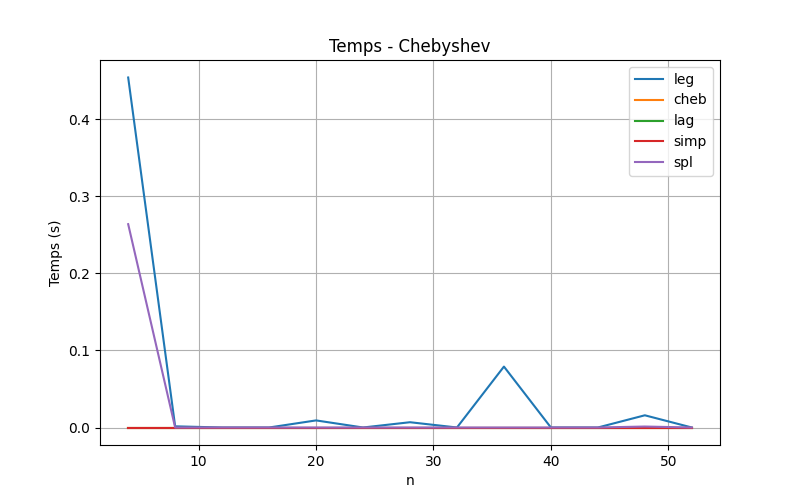
\includegraphics[width=0.65\textwidth,height=0.50\textheight,keepaspectratio]{results/graphs/Chebyshev_temps.png}
\caption{\footnotesize Temps de calcul en fonction de $n$ pour la fonction Chebyshev.}
\label{fig:cheb_temps}
\end{figure}

\vspace{-0.4cm}
\begin{block}{Commentaire}
\footnotesize
\textcolor{vert}{\textbf{Performance :}} Les méthodes de Gauss (Chebyshev, Legendre) ont un temps quasi-constant avec $n$, ce qui est optimal. La méthode Spline montre un temps plus élevé dû à la construction de l'interpolation cubique. Simpson a un temps linéaire avec $n$.
\end{block}
\end{frame}

\begin{frame}{Résultats : Fonction Laguerre - Erreurs}
\vspace{-0.3cm}
\begin{figure}[h]
\centering
\includegraphics[width=0.65\textwidth,height=0.50\textheight,keepaspectratio]{results/graphs/Laguerre_erreurs.png}
\caption{\footnotesize Évolution de l'erreur absolue pour la fonction Laguerre $f(x) = e^{-x}$ sur $[0, 20]$.}
\label{fig:lag_erreurs}
\end{figure}

\vspace{-0.4cm}
\begin{block}{Commentaire}
\footnotesize
\textcolor{bleu}{\textbf{Observation :}} Gauss-Laguerre (ligne verte) devrait théoriquement être la plus précise pour ce type d'intégrale, mais on observe que toutes les méthodes convergent bien. La méthode Spline montre une excellente précision, suivie de Simpson. L'erreur décroît rapidement avec $n$.
\end{block}
\end{frame}

\begin{frame}{Résultats : Fonction Laguerre - Temps}
\vspace{-0.3cm}
\begin{figure}[h]
\centering
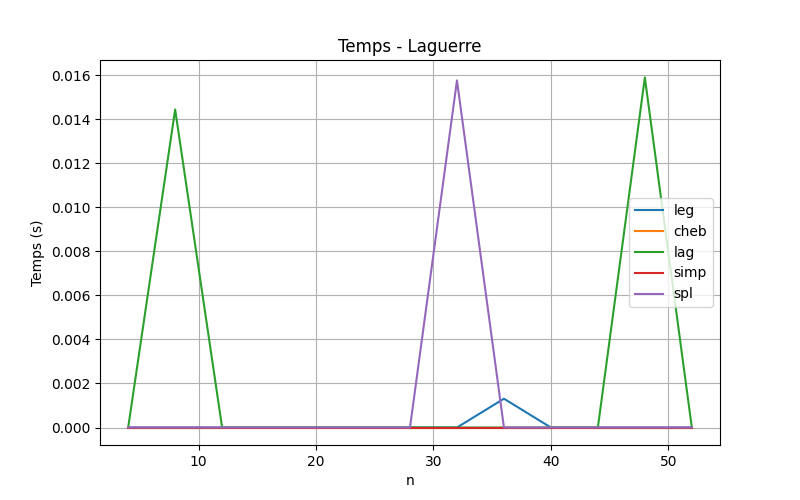
\includegraphics[width=0.65\textwidth,height=0.50\textheight,keepaspectratio]{results/graphs/Laguerre_temps.png}
\caption{\footnotesize Temps de calcul pour la fonction Laguerre.}
\label{fig:lag_temps}
\end{figure}

\vspace{-0.4cm}
\begin{block}{Commentaire}
\footnotesize
\textcolor{vert}{\textbf{Performance :}} Les temps de calcul sont similaires au cas Chebyshev. Les méthodes de Gauss restent très rapides. Pour cette fonction décroissante exponentielle, toutes les méthodes sont efficaces, avec un léger avantage aux méthodes de Gauss en termes de temps constant.
\end{block}
\end{frame}

\begin{frame}{Résultats : Fonction Mixte - Erreurs}
\vspace{-0.3cm}
\begin{figure}[h]
\centering
\includegraphics[width=0.65\textwidth,height=0.50\textheight,keepaspectratio]{results/graphs/Mixte_erreurs.png}
\caption{\footnotesize Évolution de l'erreur pour la fonction mixte $f(x) = e^{-x}/\sqrt{1-x^2}$ sur $[-0.8, 2.0]$.}
\label{fig:mixte_erreurs}
\end{figure}

\vspace{-0.4cm}
\begin{block}{Commentaire}
\footnotesize
\textcolor{rouge}{\textbf{Défi :}} Cette fonction combine les caractéristiques des deux précédentes et présente une singularité en $x=1$. Les méthodes généralistes (Simpson, Spline) montrent une meilleure robustesse. Gauss-Chebyshev et Gauss-Laguerre peuvent avoir des difficultés car elles ne sont pas optimisées pour ce cas mixte.
\end{block}
\end{frame}

\begin{frame}{Résultats : Fonction Mixte - Temps}
\vspace{-0.3cm}
\begin{figure}[h]
\centering
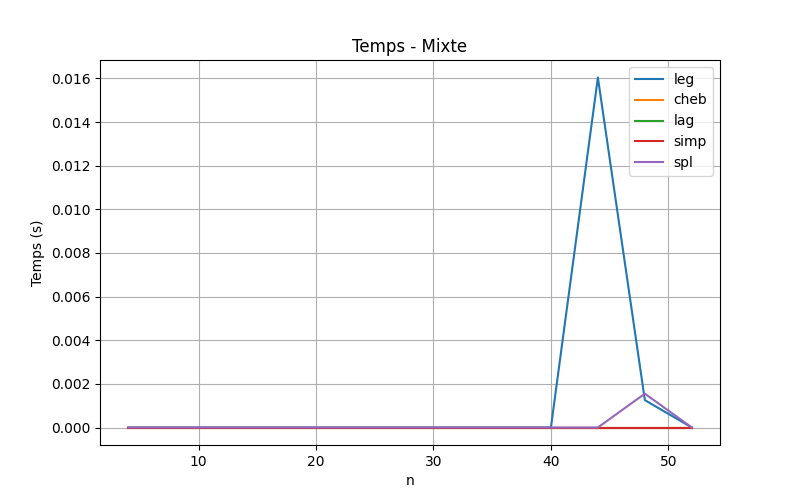
\includegraphics[width=0.65\textwidth,height=0.50\textheight,keepaspectratio]{results/graphs/Mixte_temps.png}
\caption{\footnotesize Temps de calcul pour la fonction mixte.}
\label{fig:mixte_temps}
\end{figure}

\vspace{-0.4cm}
\begin{block}{Commentaire}
\footnotesize
\textcolor{vert}{\textbf{Performance :}} Les temps restent cohérents avec les observations précédentes. La complexité de la fonction (singularité) n'affecte pas significativement le temps de calcul, mais plutôt la précision. Simpson et Spline restent les méthodes les plus robustes pour ce cas difficile.
\end{block}
\end{frame}

\begin{frame}{Résultats : Fonction Générale - Erreurs}
\vspace{-0.3cm}
\begin{figure}[h]
\centering
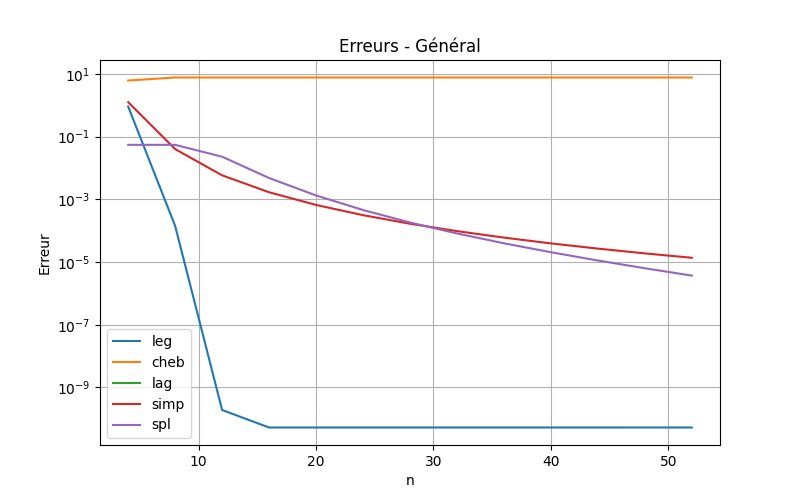
\includegraphics[width=0.65\textwidth,height=0.50\textheight,keepaspectratio]{results/graphs/Général_erreurs.png}
\caption{\footnotesize Évolution de l'erreur pour la fonction générale $f(x) = \sin(5x) + x^2$ sur $[0, 3]$.}
\label{fig:general_erreurs}
\end{figure}

\vspace{-0.4cm}
\begin{block}{Commentaire}
\footnotesize
\textcolor{bleu}{\textbf{Comparaison équitable :}} Pour cette fonction régulière sans singularités, toutes les méthodes convergent bien. Gauss-Legendre et Spline montrent les meilleures performances en précision. Simpson suit de près. C'est le cas idéal pour comparer objectivement les méthodes.
\end{block}
\end{frame}

\begin{frame}{Résultats : Fonction Générale - Temps}
\vspace{-0.3cm}
\begin{figure}[h]
\centering
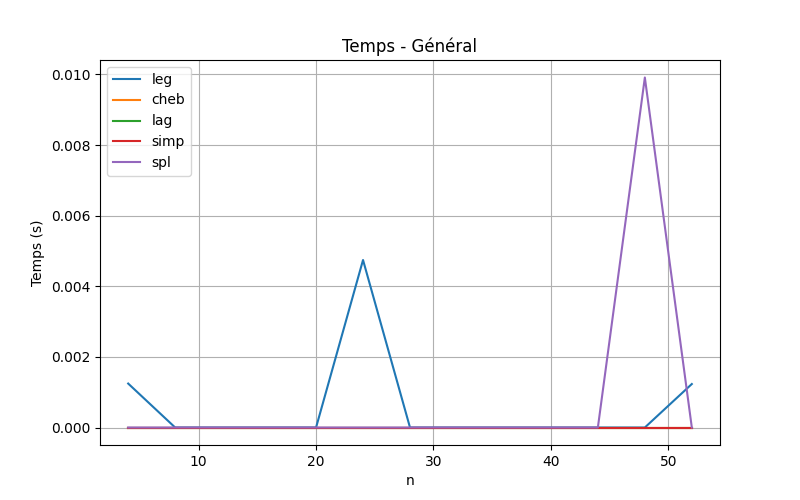
\includegraphics[width=0.65\textwidth,height=0.50\textheight,keepaspectratio]{results/graphs/Général_temps.png}
\caption{\footnotesize Temps de calcul pour la fonction générale.}
\label{fig:general_temps}
\end{figure}

\vspace{-0.4cm}
\begin{block}{Commentaire}
\footnotesize
\textcolor{vert}{\textbf{Performance :}} Les tendances sont cohérentes : méthodes de Gauss avec temps constant, Simpson linéaire, et Spline plus coûteuse. Pour une fonction régulière, le choix de la méthode peut se faire sur la base du compromis précision/temps selon les besoins de l'application.
\end{block}
\end{frame}

\subsection{Analyse des Temps}

\begin{frame}{Synthèse : Analyse des Temps de Calcul}
\vspace{-0.2cm}
\begin{block}{Tendances générales observées}
\small
\begin{itemize}
\item \textbf{Méthodes de Gauss} (Legendre, Laguerre, Chebyshev) :
\begin{itemize}
\item Temps quasi-constant avec $n$ : $O(1)$ en pratique
\item Très efficace pour des valeurs de $n$ élevées
\item Avantage : Pas de dépendance linéaire au nombre de points
\end{itemize}
\item \textbf{Simpson} :
\begin{itemize}
\item Temps linéaire : $O(n)$
\item Croissance régulière et prévisible
\item Bon compromis pour la plupart des applications
\end{itemize}
\item \textbf{Spline} :
\begin{itemize}
\item Temps plus élevé : $O(n^2)$ pour la construction
\item Nécessite plus de ressources computationnelles
\item Justifié par la précision élevée obtenue
\end{itemize}
\end{itemize}
\end{block}
\end{frame}

\subsection{Synthèse Comparative}

\begin{frame}{Tableau Récapitulatif}
\vspace{-0.3cm}
\begin{table}[h]
\centering
\tiny
\renewcommand{\arraystretch}{1.3}
\begin{tabular}{p{2.5cm}ccccp{3.5cm}}
\toprule
\textbf{Méthode} & \textbf{Précision} & \textbf{Temps} & \textbf{Robustesse} & \textbf{Domaine optimal} \\
\midrule
Gauss-Legendre & ⭐⭐⭐⭐⭐ & ⭐⭐⭐⭐ & ⭐⭐⭐ & $[a,b]$ fini \\
\midrule
Gauss-Laguerre & ⭐⭐⭐⭐⭐ & ⭐⭐⭐⭐ & ⭐⭐ & $[0,+\infty)$ \\
\midrule
Gauss-Chebyshev & ⭐⭐⭐⭐⭐ & ⭐⭐⭐⭐ & ⭐⭐ & $[-1,1]$ \\
\midrule
Simpson & ⭐⭐⭐ & ⭐⭐⭐⭐⭐ & ⭐⭐⭐⭐ & Général \\
\midrule
Spline & ⭐⭐⭐⭐ & ⭐⭐ & ⭐⭐⭐ & Fonctions lisses \\
\bottomrule
\end{tabular}
\caption{\footnotesize Comparaison qualitative des 5 méthodes d'intégration}
\label{tab:comparaison}
\end{table}

\vspace{-0.2cm}
\begin{block}{Légende}
\tiny
\begin{itemize}
\item \textbf{Précision} : Capacité à obtenir une erreur faible
\item \textbf{Temps} : Efficacité computationnelle
\item \textbf{Robustesse} : Capacité à gérer différents types de fonctions
\item \textbf{Domaine optimal} : Type d'intégrale pour lequel la méthode est conçue
\end{itemize}
\end{block}
\end{frame}

\begin{frame}{Ordre de Convergence}
\vspace{-0.2cm}
\begin{block}{Ordre théorique}
\small
\begin{itemize}
\item \textbf{Gauss-Legendre} : Ordre $2n$ (très élevé)
\item \textbf{Gauss-Laguerre} : Ordre $2n$ (très élevé)
\item \textbf{Gauss-Chebyshev} : Ordre $2n$ (très élevé)
\item \textbf{Simpson} : Ordre 4 (erreur $\sim h^4$)
\item \textbf{Spline} : Ordre 4 (erreur $\sim h^4$)
\end{itemize}
\end{block}

\vspace{-0.15cm}
\begin{block}{Observations expérimentales}
\small
\begin{itemize}
\item Les méthodes de Gauss montrent une convergence exponentielle rapide
\item Simpson et Spline montrent une convergence polynomiale d'ordre 4
\item Pour $n$ petit, les différences sont moins marquées
\item Pour $n$ grand, les méthodes de Gauss sont clairement avantageuses
\end{itemize}
\end{block}
\end{frame}

% ============================================
% SECTION 6: CONCLUSION
% ============================================
\section{Conclusion et Perspectives}

\begin{frame}{Conclusions Principales}
\vspace{-0.2cm}
\begin{block}{Méthode adaptée au problème}
\small
\begin{itemize}
\item \textbf{Pas de méthode universelle} : Le choix dépend du type de fonction
\item \textbf{Spécialisation} : Les méthodes de Gauss sont optimales dans leur domaine
\item \textbf{Robustesse} : Simpson et Spline sont plus généralistes
\end{itemize}
\end{block}

\vspace{-0.15cm}
\begin{block}{Compromis précision/temps}
\small
\begin{itemize}
\item Méthodes de Gauss : Meilleure précision, temps constant
\item Simpson : Bon compromis précision/temps pour cas généraux
\item Spline : Précision élevée mais coût computationnel important
\end{itemize}
\end{block}

\vspace{-0.15cm}
\begin{block}{Robustesse}
\small
\begin{itemize}
\item Simpson : Très robuste, fonctionne dans la plupart des cas
\item Spline : Robuste pour fonctions lisses
\item Méthodes de Gauss : Spécialisées, moins robustes mais très précises
\end{itemize}
\end{block}
\end{frame}

\begin{frame}{Recommandations}
\vspace{-0.2cm}
\begin{block}{Guide de sélection}
\small
\begin{itemize}
\item \textbf{Fonctions régulières sur $[a,b]$ fini} :
\begin{itemize}
\item $\rightarrow$ Gauss-Legendre (précision maximale)
\item $\rightarrow$ Spline (alternative précise)
\end{itemize}
\item \textbf{Domaine semi-infini $[0,+\infty)$} :
\begin{itemize}
\item $\rightarrow$ Gauss-Laguerre (méthode dédiée)
\end{itemize}
\item \textbf{Singularités aux bornes} :
\begin{itemize}
\item $\rightarrow$ Gauss-Chebyshev (si domaine $[-1,1]$)
\end{itemize}
\item \textbf{Cas général ou fonction inconnue} :
\begin{itemize}
\item $\rightarrow$ Simpson (bon compromis robustesse/précision/temps)
\end{itemize}
\end{itemize}
\end{block}
\end{frame}

\begin{frame}{Perspectives d'Amélioration}
\vspace{-0.2cm}
\begin{block}{Extensions possibles}
\small
\begin{itemize}
\item \textbf{Tests supplémentaires} :
\begin{itemize}
\item Autres types de fonctions (périodiques, discontinues)
\item Intégrales multiples
\item Intégrales avec paramètres
\end{itemize}
\item \textbf{Analyse théorique} :
\begin{itemize}
\item Démonstration rigoureuse de l'ordre de convergence
\item Estimation a priori de l'erreur
\item Optimisation du choix de $n$
\end{itemize}
\item \textbf{Optimisation} :
\begin{itemize}
\item Méthodes adaptatives (ajustement automatique de $n$)
\item Parallélisation pour temps de calcul réduit
\item Techniques d'accélération
\end{itemize}
\end{itemize}
\end{block}
\end{frame}

% ============================================
% SECTION 7: QUESTIONS
% ============================================
\section{Questions}

\begin{frame}{Questions ?}
\begin{center}
\Large
\textbf{Merci pour votre attention !}

\vspace{1cm}

\textbf{Questions et Discussion}
\end{center}

\vspace{1cm}

\begin{block}{Points de discussion possibles}
\begin{itemize}
\item Pourquoi certaines méthodes échouent sur certains domaines ?
\item Comment choisir la valeur de $n$ optimale ?
\item Complexité algorithmique détaillée
\item Méthodes adaptatives et extensions
\end{itemize}
\end{block}
\end{frame}

% ============================================
% ANNEXE (SLIDES DE BACKUP)
% ============================================
\appendix

\begin{frame}{Détails Techniques : Complexité}
\begin{block}{Complexité algorithmique}
\begin{itemize}
\item \textbf{Gauss-Legendre/Laguerre/Chebyshev} :
\begin{itemize}
\item Calcul des racines et poids : $O(n^2)$ (une seule fois, peut être précalculé)
\item Évaluation : $O(n)$
\item \textbf{Total} : $O(n)$ si précalculé, $O(n^2)$ sinon
\end{itemize}
\item \textbf{Simpson} :
\begin{itemize}
\item Évaluation de $f$ en $n+1$ points : $O(n)$
\item Calcul de la somme : $O(n)$
\item \textbf{Total} : $O(n)$
\end{itemize}
\item \textbf{Spline} :
\begin{itemize}
\item Construction de la spline : $O(n^2)$
\item Intégration : $O(n)$
\item \textbf{Total} : $O(n^2)$
\end{itemize}
\end{itemize}
\end{block}
\end{frame}

\begin{frame}{Détails Techniques : Implémentation}
\begin{block}{Bibliothèques utilisées}
\begin{itemize}
\item \texttt{numpy} : Calculs numériques, fonctions de base
\item \texttt{scipy} : Quadratures de Gauss (\texttt{leggauss}, \texttt{laggauss}), splines (\texttt{CubicSpline})
\item \texttt{matplotlib} : Génération des graphiques
\end{itemize}
\end{block}

\begin{block}{Structure du code}
\begin{itemize}
\item Architecture modulaire : séparation méthodes/exemples/calculs/visualisation
\item Gestion d'erreurs : try/except pour méthodes inadaptées
\item Réutilisabilité : fonctions génériques et paramétrables
\end{itemize}
\end{block}
\end{frame}

% ============================================
% FIN DU DOCUMENT
% ============================================
\end{document}
